\section{Eigenanalysis in R}

The \lstinline!eigen()! function computes the eigenvalues and
eigenvectors of a square matrix.

\begin{R}
> A <- matrix(c(2,1,2,3),nrow=2)
> A
     [,1] [,2]
[1,]    2    2
[2,]    1    3
> eigen.A <- eigen(A)
> eigen.A
$values
[1] 4 1
$vectors
           [,1]       [,2]
[1,] -0.7071068 -0.8944272
[2,] -0.7071068  0.4472136
> V <- eigen.A$vectors
> D <- diag(eigen.A$values) # diagonal matrix of eigenvalues
> Vinv <- solve(V)
> V %*% D %*% Vinv  # reconstruct our original matrix (see lecture slides)
     [,1] [,2]
[1,]    2    2
[2,]    1    3
> Vinv %*% A %*% V
             [,1] [,2]
[1,] 4.000000e+00    0
[2,] 2.220446e-16    1
> all.equal(Vinv %*% A %*% V, D) # test 'near equality'
[1] TRUE
> V[,1] %*% V[,2] # note that the eigenvectors are NOT orthogonal. Why?
          [,1]
[1,] 0.3162278
> B <- matrix(c(2,2,2,3),nrow=2) # define another tranformation
> B
     [,1] [,2]
[1,]    2    2
[2,]    2    3
> eigen.B$values
[1] 4.5615528 0.4384472
> eigen.B$vectors
          [,1]       [,2]
[1,] 0.6154122 -0.7882054
[2,] 0.7882054  0.6154122
> Vb <- eigen.B$vectors
> Vb[,1] %*% Vb[,2] # these eigenvectors ARE orthogonal.
     [,1]
[1,]    0
\end{R}
As we discussed in lecture, the eigenvectors of a square matrix,
$\mathbf{A}$, point in the directions that are unchanged by the
transformation specified by $\mathbf{A}$. The following relationships
relate $\mathbf{A}$ to it's eigenvectors and eigenvalues:

\[\mathbf{V}^{-1}\mathbf{A}\mathbf{V}  =  \mathbf{D} \]

\[\mathbf{A}  =  \mathbf{V}\mathbf{D}\mathbf{V}^{-1}\]
%
where $\mathbf{V}$ is a matrix where the columns represent the eigenvectors, and $\mathbf{D}$ is a diagonal matrix of eigenvalues.

Since $A$ and $B$ represent 2D transformations we can visualize the
effect of these transformations using points in the plane. We'll show
how they distort a set of points that make up a square.

\begin{R}
# define the corners of a square
> pts <- matrix(c(1,1, 1,-1, -1,-1, -1,1),4,2,byrow=T)
> pts
     [,1] [,2]
[1,]    1    1
[2,]    1   -1
[3,]   -1   -1
[4,]   -1    1
> plot(pts,xlim=c(-6,6),ylim=c(-6,6),asp=1) # plot the corners
> polygon(pts) # draw edges of square
> transA <- A %*% t(pts)
> transA
     [,1] [,2] [,3] [,4]
[1,]    4    0   -4    0
[2,]    4   -2   -4    2
> newA <- t(transA)
> newA
     [,1] [,2]
[1,]    4    4
[2,]    0   -2
[3,]   -4   -4
[4,]    0    2
> points(newA, col='red') # plot the A transformation
> polygon(newA, lty='dashed', border='red')
> newB <- t(B %*% t(pts)) # do the same for the B transformation
> polygon(newB, lty='dashed', border='blue')
> points(newB, col='blue')
> legend("topleft", c("transformation A","transformation B"),
lty=c("dashed","dashed"),col=c("red","blue"))
\end{R}
The code given above will produce the plot show in the figure below.

\begin{figure}[htbp]
\centering
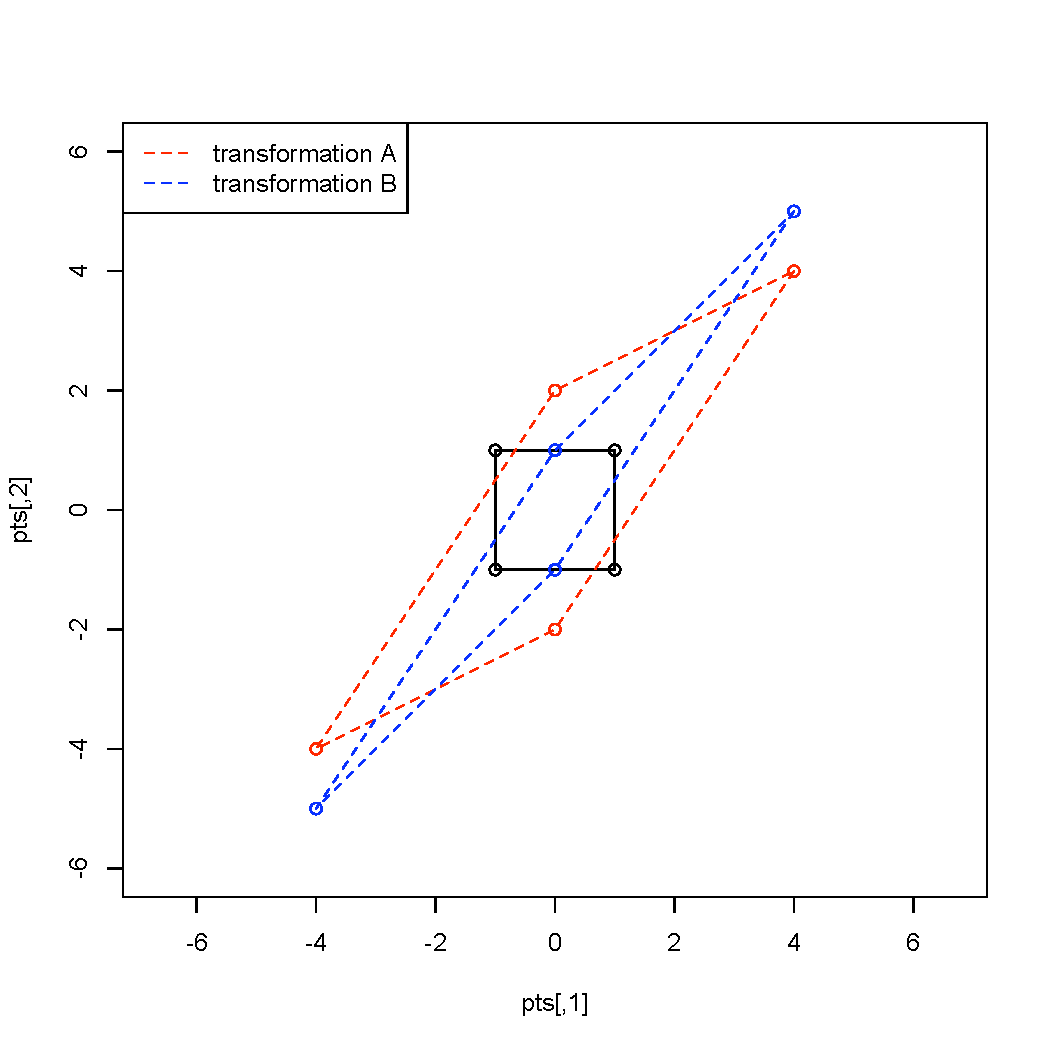
\includegraphics[width=2in]{./figures/hands-on5/eigen-transform.pdf}
\caption{Transformation of a square represented by two matrices, A and
B}
\end{figure}

\begin{assignment}
Fig.~\ref{fig:eigen} illustrates the geometry of the eigenvectors for matrices A and B as defined above.  Note that the lengths of the eigenvector depictions are scaled to be proportional to their eigenvalues. Write R code to reconstruct this figure.

\medskip

\textbf{Extra Credit:} For extra credit, write a function called |draw_eigenvector()| that will create a similar figure for any arbitrary matrix that represents a 2D transformation. Your function should tak as input a matrix $\mathbf{A}$, and a set of points in the plane.  Make sure to include code to handle cases where $\mathbf{A}$ is singular.
\end{assignment}

\begin{figure}[htbp]
\centering
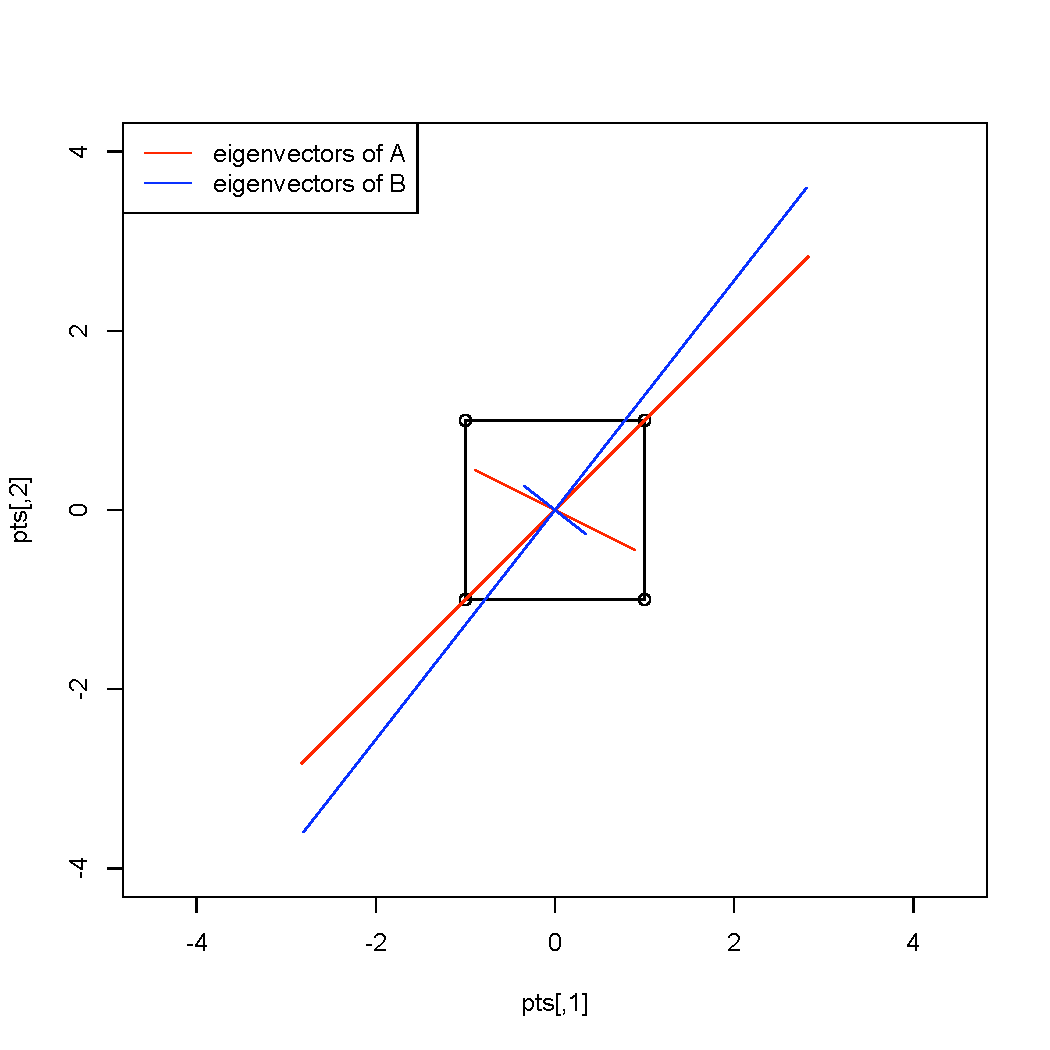
\includegraphics[width=2in]{./figures/hands-on5/eigen-ECplot.pdf}
\caption{Eigenvectors of matrices A and B \label{fig:eigen}}
\end{figure}